\documentclass[border=0.2cm]{standalone}
\usepackage{tikz}
\usetikzlibrary{calc}
\begin{document}


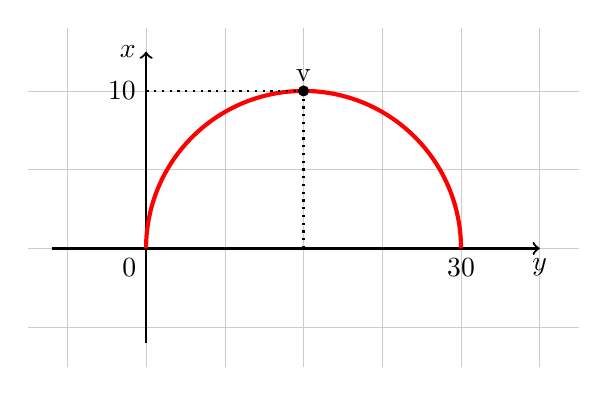
\begin{tikzpicture}
  
  \coordinate (a) at (-2,-1);
  \coordinate (b) at (2,-1);
  \coordinate (c) at (0,1);

  \draw[help lines,black!20] (-3.5,-2.5) grid (3.5,1.8);
  \draw[thick,->] (-3.2,-1) -- (3,-1) node[below] {$y$};
  \draw[thick,->] (-2,-2.2) -- (-2,1.5) node[left] {$x$};

\draw[line width=1.5pt, color=red] (-2,-1) arc (180:0:2);

\draw[thick, dotted] (c) -- +(-2,0)   node[left] {10};
\draw[thick, dotted] (c) -- +(0,-2);
\node[below] at (b) {30};
\node[below left] at (a) {0};
\fill (c) circle (2pt) node[above] {v}; 



  

  


  %\draw (-2,0) circle (1pt) node[left] {$f(x_1)$};
  %\draw (-2,1) circle (1pt) node[left] {$f(x_2)$};
  %\draw[line width=1.3pt,red] (-2.2,-2.2) -- (2,2);
  %\draw[thick, dotted] (-2,0) -- +(2,0) -- (0,-1) node[below] {$x_1$};
  %\draw[thick, dotted] (-2,1) -- +(3,0) -- (1,-1) node[below] {$x_2$};
  %\draw[thick, dotted] (0,0) -- (1,0);
  %\draw[thick] (.5,0) arc (0:45:0.5) node[right] {$\alpha$};
  %\fill (1,1) circle (1.2pt);
  %\fill (0,0) circle (1.2pt);
  
\end{tikzpicture}\\

%Este código desenha um semicírculo que começa em (0,0), termina em (4,0) e tem
%um raio de 2. No comando `arc`, os argumentos são: (-180:0:2) onde -180 é o
%ângulo de início, 0 é o ângulo final e 2 é o raio. Alternativamente, note que
%este semicírculo é desenhado ao longo do eixo x do ponto (0,0) ao ponto (4,0)
%na direção positiva.


\end{document}